\section{Method}
\label{section:method}

% The model
%-----------------------------------------------------------------------------
%   - Introduction
%   - Why iso and gyro are independent
%   - The formulas
%   - A description and reiteration in words.

% PGM
%-----------------------------------------------------------------------------
%   - The PGM
%   - A description of the PGM

% Practicalities: sampling, etc.
%-----------------------------------------------------------------------------
%   - Emcee
%   - Assessing convergence


% The model
%-----------------------------------------------------------------------------

%   - Introduction
A common approach to stellar age-dating is to make separate age predictions
using separate sets of observables.
For example, if a star's rotation period, parallax, and apparent magnitudes in
a range of bandpasses are available, it is possible to predict its age from
both gyrochronology and isochrone fitting separately.
How these two age predictions are later combined is then a difficult choice.
Is it best to average these predictions or just use the more precise of the
two, or the one believed to be more accurate?
The methodology described here provides an objective method for combining age
estimates.
There is, after all, only one age for each star.
% If the two or more dating methods do not agree on the same age then one or
% models must be inaccurate.
% More words about the implications of this.
In Bayesian statistics, combining information from different models can be
relatively simple, as long as the processes being modeled; those that
generated the data, are independent.
In this case, we are combining information that relates to the burning of
hydrogen in the core (this is the process that drives the slow increase in
\teff\ and luminosity over time) with information about the magnetic braking
history of a star (the current rotation period).
We can assume that, to first order, these two processes are independent: the
hydrogen fraction in the core does not affect a star's rotation period and
vice versa.
In practise,  we can never be entirely sure that two such processes are
independent but, at least within the uncertainties, any dependence here is
unlikely to affect our results.
If this assumption is valid, the likelihoods calculated using each model can
be multiplied together.

The desired end product of this method is an estimate of the non-normalized
posterior probability density function (PDF) over the age of a star,
\begin{equation} p(A|{\bf m_x}, T_{\mathrm{eff}}, \log g, \hat{F}, P,
    \bar{\omega}), \end{equation} where $A$ is age, ${\bf m_x}$ is a vector of
apparent magnitudes in various bandpasses (in our model ${\bf m_x} =
[m_J,~m_H,~m_K]$), \fhat\ is the {\it observed} bulk metallicity, $P$ is
the rotation period and \pmega\ is parallax.
In order to calculate a posterior PDF over age, we must marginalize over
parameters that relate to age, but are not of interest in this study: mass
($M$), distance ($D$), V-band extinction ($A_V$) and the {\it inferred} bulk
metallicity, $\mathrm{F}$.
The marginalization involves integrating over these extra parameters,
\begin{eqnarray}
& p(A|{\bf m_x}, T_{\mathrm{eff}}, \log g, \hat{F}, P, \bar{\omega})
\\ \nonumber
& \propto \int p({\bf m_x}, T_{\mathrm{eff}}, \log g, \hat{F}, P, \bar{\omega}|
A, M, D, A_V, F)~p(A)p(M)p(D)p(A_V)p(F)
dMdDdA_VdF.
\label{eqn:bayes}
\end{eqnarray}
This equation is a form of Bayes' rule,
\begin{equation}
\mathrm{Posterior} \propto \mathrm{Likelihood} \times \mathrm{Prior},
\end{equation}
where the likelihood of the data given the model is,
\begin{equation}
p({\bf m_x}, T_{\mathrm{eff}}, \log g, \hat{F}, P, \bar{\omega}|A, M, D,
A_V, F),
\end{equation}
and the prior PDF over parameters is,
\begin{equation}
p(A)p(M)p(D)p(A_V)p(F).
\label{eqn:prior}
\end{equation}

%   - Why iso and gyro are independent.
Not all of the observables on the left of the `$|$' in the likelihood depend
on all of the parameters to the right of it.
For example, rotation period, $P$ doesn't depend on V-band extinction, $A_V$.
In our model, we make use of conditional independencies like this and use them
to factorize the likelihood.
Instead of the likelihood we wrote in equation \ref{eqn:bayes},
where every observable depends on every parameter, our model can be factorized
as,
\begin{equation}
    p({\bf m_x}, T_{\mathrm{eff}}, \log g, \hat{F}, \bar{\omega}, C_{B-V}|A,
    M, D, A_V, F)
    ~p(P|A, C_{B-V}),
\label{eqn:factorized}
\end{equation}
where we have introduced a new parameter, $C_{B-V}$, which is the $B-V$ color
that is often used as a mass proxy in the literature.
In our model $C_{B-V}$ is not measured but {\it inferred}: it is a latent
parameter.
We infer $C_{B-V}$ because all \kepler\ stars have 2MASS photometry in J, H
and K bands but do not all have B and V band colors.
However, the gyrochronology model we use is calibrated to B-V color, not J-K
or otherwise.
A probabilistic graphical model (PGM) depicting the joint probability over
parameters and observables is shown in figure \ref{fig:PGM}.
It describes the conditional dependencies between parameters (in white
circles) and observables (in grey circles) with arrows leading from the causal
processes to the dependent processes.
For example, it is the mass, age, metallicity, extinction and distance that
determines the observed spectroscopic properties (\teff, \logg\ and \feh)
and apparant magnitudes ($m_J$, $m_H$ and $m_K$).
These parameters also determine the B-V color of a star.
In turn, it is a star's age and B-V color that determine its rotation period.
Note that, written this way, stellar rotation periods do not directly depend
on stellar mass.
Mass determines $C_{B-V}$ and $C_{B-V}$, along with age determines rotation
period.
The purpose of this PGM is not to depict the physical realities of stellar
evolution, it is only a visual description of the structure of the model {\it
we} use here.
Braking up the problem this way allows us to efficiently join isochronology
and gyrochronology and infer the joint age of a star from all its observables.
It may well be that rotation period depends directly on mass and metallicity
in reality, but it is more practical for us to assume that these dependencies are
weak enough not to significantly affect the ages that we ultimately infer.

% The PGM
\begin{figure}
  \caption{
A probabilistic graphical model (PGM) showing the conditional
dependencies between the parameters (white nodes) and
observables (gray nodes) in our model.
Apparent magnitude, $m_x$, effective temperature, \teff, surface gravity,
\logg, observed bulk metallicity, $\hat{F}$, and parallax, $\bar{\omega}$ are
determined by the mass, $M$, age, $A$, distance, $D$, extinction, $A_V$
and bulk metallicity, $F$, of a star.
These dependencies are indicated by arrows that start at a `parent' node
and end at the dependent observable, or `child' node.
The box drawn around some of the nodes indicates that everything inside it
depends on every parameter that points toward it.
For example, \logg\ depends on $A$, $M$, $D$, $A_V$, and $F$.
In our model, rotation period, $P$, only depends on age and a
B-V color that is a latent parameter, predicted from the isochronal model.
In our model, rotation period does not directly depend on distance,
extinction, metallicity or mass, only age and B-V color.
This PGM is a representation of the factorized joint PDF over parameters and
observables which is written in equation \ref{eqn:joint}.
}
  \centering
    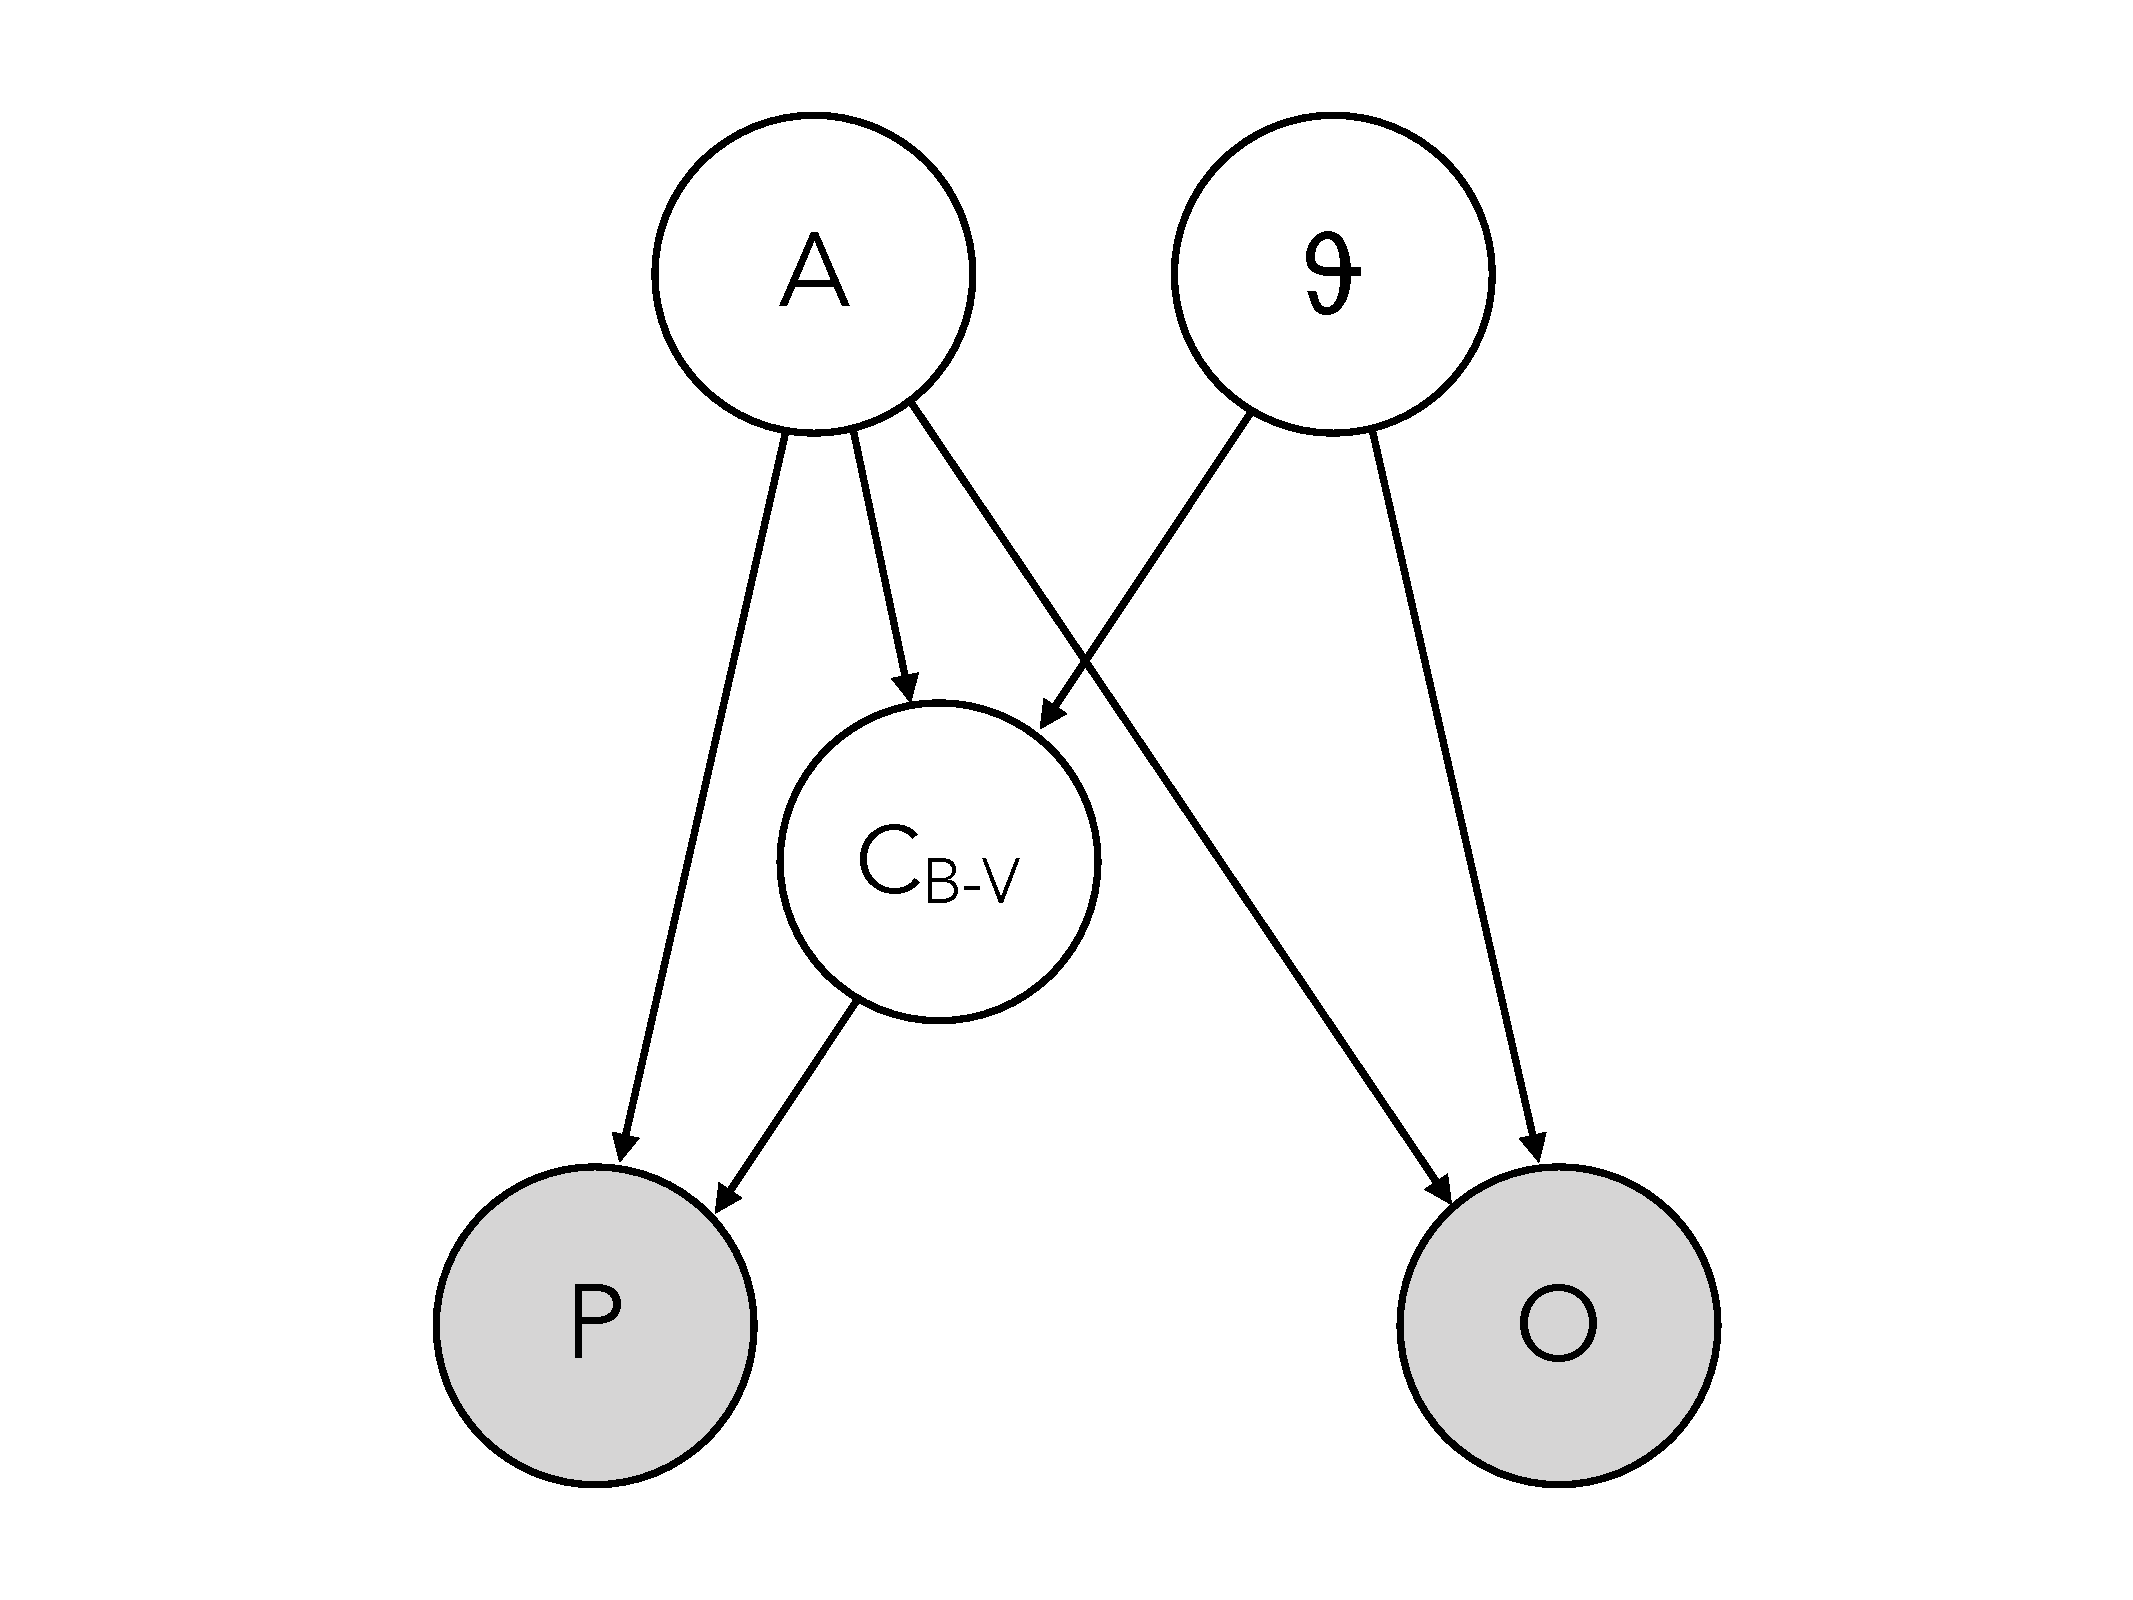
\includegraphics[width=.7\textwidth]{PGM}
\label{fig:PGM}
\end{figure}

%   - The formulas
The factorization of the likelihood described in equation \ref{eqn:factorized}
and depicted in figure \ref{fig:PGM} allows us to multiply two separate
likelihood functions together: one computed using an isochronal model and one
computed using a gyrochronal model.
We assume that the probability of observing the measured observables, given
the model parameters is a Gaussian and that the observables are identically
and independently distributed.
These assumptions allow us to use Gaussian likelihood functions.
The isochronal likelihood function is,
\begin{eqnarray}
    & \mathcal{L_{\mathrm{iso}}} = p({\bf m_x}, T_{\mathrm{eff}}, \log g, \hat{F},
    \bar{\omega}, C_{B-V}|A, M, D,
    A_V, F) \\ \nonumber
    & = \frac{1}{\sqrt{(2\pi)^n \det(\Sigma)}}
    \exp\left( -\frac{1}{2} ({\bf O_I} - {\bf I})^T \Sigma ^{-1}
    ({\bf O_I} - {\bf I})\right),
\label{eqn:iso_likelihood}
\end{eqnarray}
where ${\bf O_I}$ is the vector of $n$ observables: \teff, \logg, \fhat,
\pmega, \mj, \mh\ and \mk and $\Sigma$ is the covariance matrix of that set of
observables.
${\bf I}$ is the vector of {\it model} observables that correspond to a set of
parameters: $A$, $M$, $F$, $D$ and $A_V$, calculated using an isochrone model.
We assume there is no covariance between these observables and so this
covariance matrix consists of individual parameter variances along the
diagonal with zeros everywhere else.
The gyrochronal likelihood function is,
\begin{eqnarray}
    & \mathcal{L_{\mathrm{gyro}}} = p(P |A, C_{B-V}) \\ \nonumber
    & = \frac{1}{\sqrt{(2\pi) \det(\Sigma_P)}}
    \exp\left( -\frac{1}{2} ({\bf P_O} - {\bf P_P})^T \Sigma ^{-1}
    ({\bf P_O} - {\bf P_P})\right),
    % = \prod_i \frac{1}{\sqrt{2\pi}\sigma_i} \exp
    % \left(-\frac{(P_{\mathrm{obs}, i} - P_{\mathrm{pred},
    % i})^2}{2\sigma_i^2}\right),
\label{eqn:gyro_likelihood}
\end{eqnarray}
% where $P_{\mathrm{obs}, i}$ is the $i$th observed rotation period,
% $P_{\mathrm{pred}, i}$ is the corresponding predicted rotation period,
% calculated from the $i$th age and $C_{B-V}$ values predicted by the isochronal
% model.
where ${\bf P_O}$ is a 1-D vector of observed rotation periods, ${\bf P_P}$ is
the vector of corresponding predicted rotation periods, calculated using the
vector of inferred ages and $C_{B-V}$ values predicted by the isochronal
model.
The full likelihood function used in our model is the product of these two
likelihood functions,
\begin{eqnarray}
    & \mathcal{L_{\mathrm{full}}} = \frac{1}{\sqrt{(2\pi)^n \det(\Sigma)}}
    \exp\left( -\frac{1}{2} ({\bf O_I} - {\bf I})^T \Sigma ^{-1}
    ({\bf O_I} - {\bf I})\right) \\ \nonumber
    & \times
    \frac{1}{\sqrt{(2\pi) \det(\Sigma_P)}}
    \exp\left( -\frac{1}{2} ({\bf P_O} - {\bf P_P})^T \Sigma ^{-1}
    ({\bf P_O} - {\bf P_P})\right).
\label{eqn:full_likelihood}
\end{eqnarray}

%   - Priors
We place priors over the model parameters $A$, $M$, $F$, $D$ and $A_V$.
These priors represent our `prior beliefs' about the values these parameters
will take, before we use the data to update those beliefs via a likelihood and
produce a `posterior' belief about their values.
These priors are described in the appendix.

%   - A word about the gyrochronology model.
We use a three-dimensional polynomial model to predict rotation period as a
function of \gaia\ color and age.
This model consists of a 4th order polynomial in logarithmic Gaia color:
$G_{Bp} - G_{Rp}$, which we write as $C_G$ for simplicity, and a 1st order
polynomial (a straight line) in logarithmic age.
\begin{equation}
    \log(P) = a + b\log(C_G) + c\log^2(C_G) + d\log^3(C_G) + e\log^4(C_G)
    + f\log(A)
\label{eqn:gyro}
\end{equation}
where $P$ is rotation period in days, $C_G$ is Gaia color, $A$ is stellar age
in years and the lower case letters are free parameters which we fit to the
data using linear least squares.
A more detailed description of this process is provided in section
\ref{section:results}.

In \citet{angus2015} it was found that the old asteroseismic stars could not
be fit using a single power law in age.
Subsequently, \citet{vansaders2016} discovered that the magnetic braking of
these old stars has ceased and cannot be modeled with a Skumanich-like
spin-down law.
In future, the above model should be updated to include a more flexible
treatment of rotation period as a function of age in order to account for the
change in slope of the rotation period-age relation.
Until then, this method should only be used for stars below the Rossby number
threshold, \ie\ who's rotation period to convection overturn time ratio
($P/\tau = Ro$) does not exceed 2.1 \citep{vansaders2016}.
In this work we are chiefly concerned with introducing a new framework where
rotation periods are modeled {\it simultaneously} with isochronal features.
Although this gyrochronology model does not provide a good fit to all the
available data, we reiterate that no single model {\it is} able to reproduce
all the data, and that there is utility in using such a simple, linear,
empirical model like this.
Again, we are not particularly attempting to improve gyrochronology models in
this work: in this paper we are more concerned with introducing a new approach
to modeling stellar ages, however, our method is highly flexible and modular
and an improved gyrochronology model could easily be swapped in for this one
in future.

The Sun's color in the Gaia color bandpasses, $G_{Bp} - G_{Rp}$, is 0.82
\citep{casagrande2018}.

% Practicalities: sampling, etc.
%-----------------------------------------------------------------------------
%- isochrones.py
To calculate ${\bf I}$, the vector of predicted isochronal observables, we use
the {\tt isochrones.py} {\it python} package which has a range of
functionalities relating to isochrone fitting.
The first of the {\tt isochrones.py} functions we use is the likelihood
function of equation \ref{eqn:iso_likelihood}.
The {\tt isochrones.py} likelihood function accepts a dictionary of
observables which can, but does not {\it have} to include, all of the
following: \teff, \logg, \feh, parallax and apparent magnitudes in a range of
colors, as well as the uncertainties on all these observables.
It then calculates the residual vector $({\bf O_I} - {\bf I})$ where ${\bf
O_I}$ is the vector of observables and ${\bf I}$ is a vector of corresponding
predicted observables.
The prediction is calculated using a set of isochrones \citep[we use the MIST
models][]{choi}, where the set of {\it model} observables that correspond to a
set of physical parameters is returned.
This requires interpolation over the model grids since, especially at high
dimensions, it is unlikely that any set of physical parameters will exactly
match a precomputed set of isochrones.
The observables that correspond to a set of physical parameters (age, mass,
etc) go into ${\bf I}$ and the {\tt isochrones.py} likelihood function returns
the result of equation \ref{eqn:iso_likelihood}.
The second {\tt isochrones.py} function we use is one that querys the best-fit
isochrone model chosen to predict ${\bf I}$, in order to predict the
corresponding $C_{B-V}$ for that star.
This color is then used to calculate the gyrochronal likelihood function of
equation \ref{eqn:gyro_likelihood}.

%   - Step-by-step description
The inference processes procedes as follows (as a reminder, we use {\it
observables} to refer to the data: \teff, \logg, etc and {\it parameters} to
refer to the model parameters: age, mass, etc).
First, a set of parameters: age, mass, true bulk metallicity, distance and
extinction, as well as observed values of \teff, \logg, bulk metallicity,
2MASS colors and parallax (${\bf O_I}$) for a single star are passed to the
isochronal likelihood function (equation \ref{eqn:iso_likelihood}).
Then, a set of {\it model} values of \teff, \logg, bulk metallicity, 2MASS
colors and parallax (${\bf I}$) that correspond to that set of parameters are
calculated by {\tt isochrones.py}.
The isochronal log-likelihood, $\ln(\mathcal{L}_{\mathrm{iso}})$, is then
computed for these parameter values.
The same age that was passed to the likelihood function, and the $C_{B-V}$
corresponding to it, along with the observed rotation period, are then passed
to the gyrochronal likelhood function (equation \ref{eqn:gyro_likelihood}).
The gyrochronal log-likelihood, $\ln(\mathcal{L}_{\mathrm{gyro}})$, is
computed.
The full log-likelihood is then calculated: $\ln(\mathcal{L}_{\mathrm{full}})
= \ln(\mathcal{L}_{\mathrm{iso}}) + \ln(\mathcal{L}_{\mathrm{gyro}})$ and
added to the log-prior to produce a single sample from the posterior PDF.

%   - Emcee, including assessing convergence.
We sampled the joint posterior PDF over age, mass, metallicity, distance and
extinction using the affine invariant ensemble sampler, {\tt emcee}
\citep{foreman-mackey2013}.
We used 24 walkers and sampled the posterior PDF until 100 {\it independent}
samples were obtained.
We estimated the autocorrelation length, indicating how many steps are taken
per independent sample, after every 100 steps using the autocorrelation tool
built into {\tt emcee}.
We stopped obtaining samples when either {\it both} 100 times the
autocorrelation length was reached {\it and} the change in autocorrelation
length over 100 samples was less than 0.01, or the maximum of 100,000 samples
was obtained.
This allowed use to continue obtaining samples from the posterior
This provided an average of ... non-independent samples.
The method described above is trivially parallelizable, since the
inference proccess for each star can be inferred on a separate node.
Running our code on a cluster, we found that a posterior PDF can be estimated
for a single star in around one minute.
